The sole purpose of this layer is to control the Turning Board. This layer is directly accessible to the user. This remote is in the form of an android app or IOS app. This layer communicates with the Main Control layer adequately to propagate user commands. Some features included in this layer include: user authentication, and user ride data analysis.

\subsection{Layer Hardware}
The remote controller for the Turing board is an app, which can be a acquired from an app store. This app runs on a smart phone capable to downloading apps.


\subsection{Layer Operating System}
The remote app can run on Android or IOS.

\subsection{Layer Software Dependencies}
The UI is connected to a Firebase back-end, which includes of a real-time NoSQL database

\subsection{Front-end UI and Main Control communication}
The front-end UI is what the user sees on the Turing board's app. The app is used as a remote controller for the Turing board. This is where different riding modes are selected. It is also where authentication and data analysis happens. The app communicates with our firebase back-end which in turn communicates with the control layer, our embedded computer. The control layer then propages the commands to the appropriate hardware.

%%%%%%%%%%%%%%%%%%%%%%%%%%%%%%%%%%%%%%%%%%%%%%%%%%%%%%%%%%
%  BE SURE TO UPDATE THE IMAGE CAPTION
\begin{figure}[h!]
	\centering
 	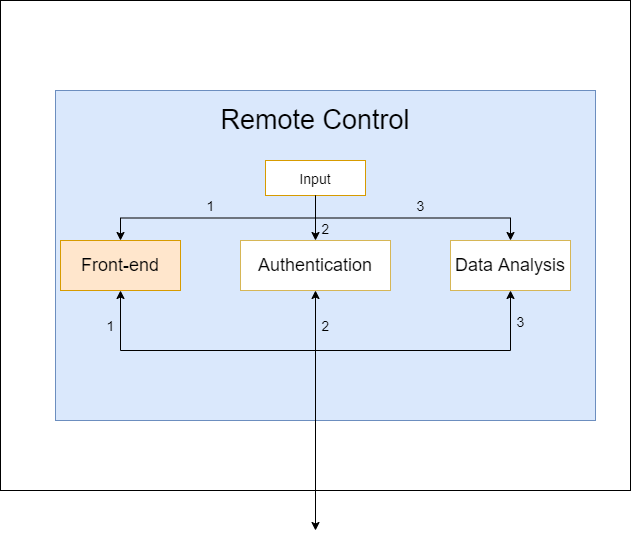
\includegraphics[width=0.60\textwidth]{DDS/images/UIJetsonCom.png} % Image
 \caption{Front-end UI and Main Control communication diagram} % Caption
\end{figure}

\subsubsection{Subsystem Hardware}
This system is accessed through the remote controller app, which requires a smartphone to run on.

\subsubsection{Subsystem Operating System}
Android or IOS is required to run the controller app

\subsubsection{Subsystem Software Dependencies}
The front-end UI and Main Control communication subsystem depends on Wifi and a firebase back-end.

\subsubsection{Subsystem Programming Languages}
React-native and JavaScript 

\subsubsection{Subsystem Data Structures}
The data from the Front-end UI and Main Control communication subsystem is received and sent to the back end as JSON objects

\subsubsection{Subsystem Data Processing}
N/A

\subsection{Ride Data Analysis}
This sub layer of the remote controller layer will be information provided to the user after a ride. This information may include average speed of the ride, the duration of the ride, and the distance traveled. This information will be displayed on the app.

%%%%%%%%%%%%%%%%%%%%%%%%%%%%%%%%%%%%%%%%%%%%%%%%%%%%%%%%%%
%  BE SURE TO UPDATE THE IMAGE CAPTION
\begin{figure}[h!]
	\centering
 	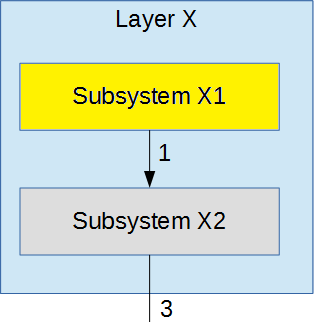
\includegraphics[width=0.60\textwidth]{images/subsystem} % Image
 \caption{Ride Data Analysis subsystem diagram} % Caption
\end{figure}

\subsubsection{Subsystem Hardware}
N/A

\subsubsection{Subsystem Operating System}
This feature is within the controller app, so it runs on Android and IOS

\subsubsection{Subsystem Software Dependencies}
The Ride Data Analysis subsystem depends on the controller app, and on a firebase NoSQL database.

\subsubsection{Subsystem Programming Languages}
React and JavaScript 

\subsubsection{Subsystem Data Structures}
The data from the Ride Data Analysis subsystem is received from the back-end as JSON objects

\subsubsection{Subsystem Data Processing}
N/A

\subsection{Authentication}
When the user attempt to log into the app or sign up, the UI parses the login/signup information (name, email, password, etc.) the parsed data is then sent to a Firebase authentification API. The API in turn forwards a token to the app confirming status of the attempt, either successful or unsuccessful login/sign up. The app then uses the data to render the UI accordingly.

%%%%%%%%%%%%%%%%%%%%%%%%%%%%%%%%%%%%%%%%%%%%%%%%%%%%%%%%%%
%  BE SURE TO UPDATE THE IMAGE CAPTION
\begin{figure}[h!]
	\centering
 	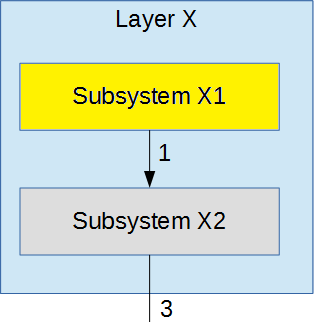
\includegraphics[width=0.60\textwidth]{images/subsystem} % Image
 \caption{Authentication subsystem diagram} % Caption
\end{figure}

\subsubsection{Subsystem Hardware}
N/A

\subsubsection{Subsystem Operating System}
N/A

\subsubsection{Subsystem Software Dependencies}
The Authentication subsystem depends on the app, and on the firebase authentication API.

\subsubsection{Subsystem Programming Languages}
The front-end is written using React-native and JavaScript 

\subsubsection{Subsystem Data Structures}
The data from the Authentication subsystem is being sent to the back end as JSON objects

\subsubsection{Subsystem Data Processing}
N/A

% \subsection{Ride Data Analysis}
% This sub layer of the control layer will be information provided to the user after a ride. This information may include average speed of the ride, the duration of the ride, and the distance traveled.

% %%%%%%%%%%%%%%%%%%%%%%%%%%%%%%%%%%%%%%%%%%%%%%%%%%%%%%%%%%
% %  BE SURE TO UPDATE THE IMAGE CAPTION
% \begin{figure}[h!]
% 	\centering
%  	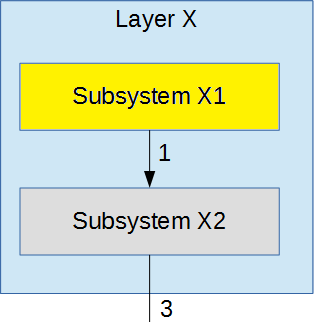
\includegraphics[width=0.60\textwidth]{images/subsystem} % Image
%  \caption{Example subsystem description diagram} % Caption
% \end{figure}

% \subsubsection{Subsystem Hardware}
% N/A

% \subsubsection{Subsystem Operating System}
% This feature is within the controller app, so it runs on Android and IOS

% \subsubsection{Subsystem Software Dependencies}
% The Ride Data Analysis subsystem depends on the controller app, and on firebase NoSQL database.

% \subsubsection{Subsystem Programming Languages}
% React and JavaScript 

% \subsubsection{Subsystem Data Structures}
% The data from the Ride Data Analysis subsystem is received from the back-end as JSON objects

% \subsubsection{Subsystem Data Processing}
% N/A

% \subsection{Ride Data Analysis}
% This sub layer of the control layer will be information provided to the user after a ride. This information may include average speed of the ride, the duration of the ride, and the distance traveled.

% %%%%%%%%%%%%%%%%%%%%%%%%%%%%%%%%%%%%%%%%%%%%%%%%%%%%%%%%%%
% %  BE SURE TO UPDATE THE IMAGE CAPTION
% \begin{figure}[h!]
% 	\centering
%  	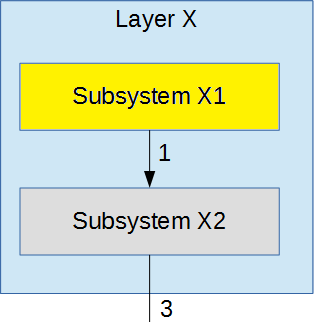
\includegraphics[width=0.60\textwidth]{images/subsystem} % Image
%  \caption{Example subsystem description diagram} % Caption
% \end{figure}

% \subsubsection{Subsystem Hardware}
% N/A

% \subsubsection{Subsystem Operating System}
% This feature is within the controller app, so it runs on Android and IOS

% \subsubsection{Subsystem Software Dependencies}
% The Ride Data Analysis subsystem depends on the controller app, and on firebase NoSQL database.

% \subsubsection{Subsystem Programming Languages}
% React and JavaScript 

% \subsubsection{Subsystem Data Structures}
% The data from the Ride Data Analysis subsystem is received from the back-end as JSON objects

% \subsubsection{Subsystem Data Processing}
% N/A
